\documentclass[10pt, twoside, a4paper]{article}
\usepackage[italian]{babel}
\usepackage[utf8]{inputenc}
\usepackage{amsmath}
\usepackage{amsfonts}
\usepackage{fullpage}
\usepackage[pdftex]{graphicx}
\usepackage{booktabs}
\usepackage{wrapfig}
\usepackage{multirow}
\usepackage{sidecap}
\usepackage{subcaption}
\usepackage{siunitx}
\usepackage[font=small]{caption}
\usepackage[bookmarks, hidelinks]{hyperref}
\usepackage{float}
%nuovi pacchetti
\usepackage{fontenc}
\usepackage{fancyhdr}
\usepackage{amssymb}
\usepackage{enumitem}
\usepackage [a4paper, top=1.4cm, bottom=1.4cm, left=1.5cm, right=1.5cm] {geometry}
\usepackage{multicol}

\begin{document}

\begin{center}

     	{\huge Amplificatori operazionali}

     	\vspace{0.2cm}
	\vspace{0.3cm}

      	{\large Alessandro Martinelli, Davide Bazzanella} \\
%     	{Bazzanella.Davide@gmail.com} \\
		{ Gruppo B10} \\
	
	\vspace{0.1cm}
      	{ 27 maggio 2014 }

\end{center}

Mediante l'oscilloscopio, verificare la funzione di trasferimento per filtri passa basso, passa banda e reiezione di banda.\begin{wrapfigure}[6]{r}[0pt]{130mm}
	\centering
    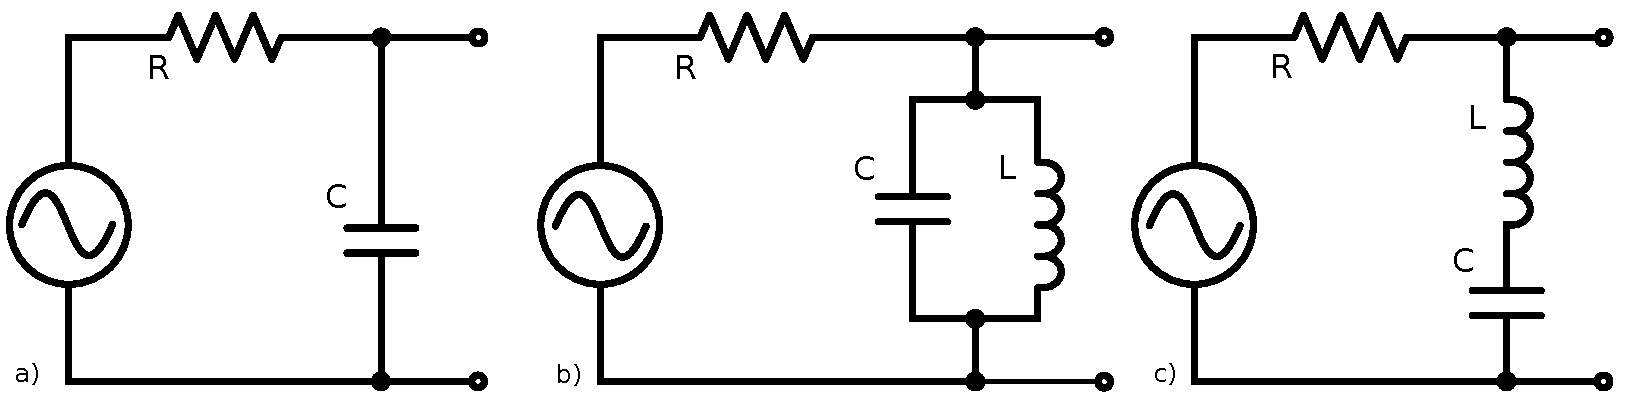
\includegraphics[width=0.7\textwidth]{circuiti.pdf}
    \caption{Schema dei circuiti utilizzati: a) filtro passa basso; b) filtro passa banda; c) filtro a reiezione di banda}
    \label{fig:circuito}
\end{wrapfigure}

\section{Strumenti}

$\bullet \quad$Oscilloscopio \\
$\bullet \quad$Cablaggio\\
$\bullet \quad$Breadboard (basetta sperimentale)\\
$\bullet \quad$Generatore di forme d'onda\\
$\bullet \quad$Multimetro digitale\\
$\bullet \quad$Decadi di resistenze,\\
\hspace{20pt} capacitori e induttanze\\

\section{Amplificatore invertente e non-invertente}

\begin{figure}[h!]
\centering
		\begin{minipage}[c]{.4\textwidth}
			\centering

			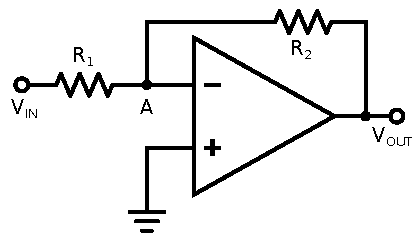
\includegraphics[width=.65\textwidth]{ccinv.pdf}
			\label{fig:ccinv}
			\caption{Amplificatore invertente}

		\end{minipage}%
		\hspace{10mm}%
		\begin{minipage}[c]{.4\textwidth}
			\centering

			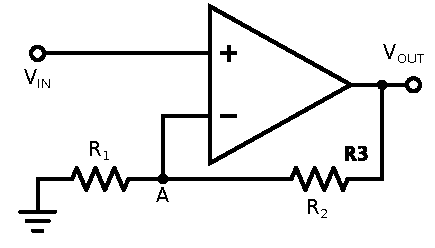
\includegraphics[width=.65\textwidth]{ccninv.pdf}
			\label{fig:ccninv}
			\caption{Amplificatore non invertente}
			
		\end{minipage}
\end{figure}

Il primo circuito da noi analizzato consiste in un amplificatore invertente accoppiato DC.
Lo schema è riportato in Fig.(\ref{fig:ccinv}).
Come vediamo, il nostro amplificatore operazionale è collegato con un circuito di \textbf{feedback} \textbf{negativo} (ovvero viene portato un po' del segnale in output all'ingresso invertente).
Così facendo possiamo avere un controllo sul segnale in uscita che altrimenti sarebbe, per come è costruito l'op-amp, $\pm V$ (avendo un guadagno di $10^6$).

Se consideriamo il nostro amplificatore operazionale ideale, abbiamo che $\Delta V_{12}=0$ (prima condizione di idealità).
Il punto $A$ sarà un ground virtuale.
Possiamo dunque imporre $I_1=\frac{V_{in}-V_A}{R_1}=\frac{V_{in}}{R_1}$.
Inoltre $I_2=\frac{V_A-V_{out}}{R_2}=\frac{-V_{out}}{R_2}$.
Sfruttando la seconda condizione di idealità, $\Delta I_{12}=0$, otteniamo $V_{out}=-\frac{R_2}{R_1} V_{in}$.
Il guadagno del nostro circuito amplificatore sarà dunque:

$$G=-\frac{R_2}{R_1}$$

Esso è negativo in quanto sfasato rispetto al segnale in ingresso di $\pi$.
La richiesta fatta era di ottenere un guadagno di circa -10.
Abbiamo dunque scelto di usare $R_1=(1001.6\pm0.3)\Omega$ e $R_2=(9987.1\pm0.3)\Omega$.
Il circuito è stato alimentato con un segnale in input sinusoidale alla frequenza di 1kHz.
Per valori picco-picco maggiori di $3V$ abbiamo notato l'ormai classico effetto di clapping del segnale, in quanto la tensione in output raggiungeva il valore massimo fornito dalla polarizzazione DC dell'op-amp. 

Ne abbiamo inoltre analizzato l'andamento al variare della frequenza.
Come già accaduto per l'amplificatore alle differenze, abbiamo notato che a frequenze elevato il guadagno diminuiva considerevolmente, con anche uno sfasamento rilevante dei segnali.
In Fig.(\ref{fig:ccninv}) è riportato un grafico del guadagno in funzione della frequenza. 

$$Grafico??$$

$$Se abbiamo i dati$$


Crediamo che il motivo di tale smorzamento del segnale sia la presenza dei transistor e delle capacità nell'amplificatore operazionale.


Successivamente abbiamo montato l'amplificatore non invertende come mostrato in Fig.(\ref{fig:ccninv}). Con gli stessi ragionamenti fatti sopra, possiamo calcolare il guadagno di tale circuito: $V_A=V_{in}=V_{out}\frac{R_1}{R_2+R_1} \Rightarrow V_{out}=(1+\frac{R_2}{R_1})$. Il guadagno, positivo in questo caso, risulta essere: 

$$G=1+\frac{R_2}{R_1}$$

Anche per questo circuito abbiamo analizzato la risposta in frequenza.
Il risultato ottenuto è identico a quello per il circuito precedentemente analizzato e dunque abbiamo deciso di non riportare un grafico.
\section{Sommatore}

\begin{wrapfigure}[12]{r}[0pt]{65mm}
	\caption{Circuito sommatore}
	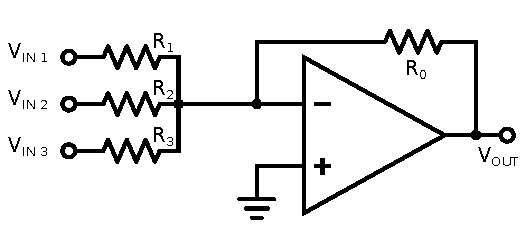
\includegraphics[width=65mm]{ccsum.pdf}
	\label{fig:ccsum}
\end{wrapfigure}

Il circuito riportato in Fig.(\ref{fig:ccsum}) è lo schema del circuito sommatore.
Tale circuito permette di sommare più segnali in input e risulta particolarmente comodo nel caso, ad esempio, della necessità di trasformare un segnale digitale (espresso in bit) in un segnale analogico (ampiezza).
Analizziamo il circuito sempre assumendo un op-amp ideale.
Anche in questo caso $V_A$ sarà un ground virtuale ($V_A = 0$).
Possiamo dunque imporre la seguente condizione: $\frac{V_1}{R_1}+\frac{V_2}{R_2}+\frac{V_3}{R_3}=\frac{-V_{out}}{R_0}$.
Dunque, se $R_0=R_1=R_2=R_3$ segue immediatamente che $V_{out}=-(V_1+V_2+V_3)$.
Ne abbiamo verificato il funzionamento utilizzando diversi segnali in input (tra cui onde quadre, segnali DC, ecc.).

Nei seguenti grafici in Fig. \ref{fig:sum} sono riportati i segnali visualizzati a schermo sull'oscilloscopio per alcune combinazioni di segnali in input.

\begin{figure}[h]
	\centering
			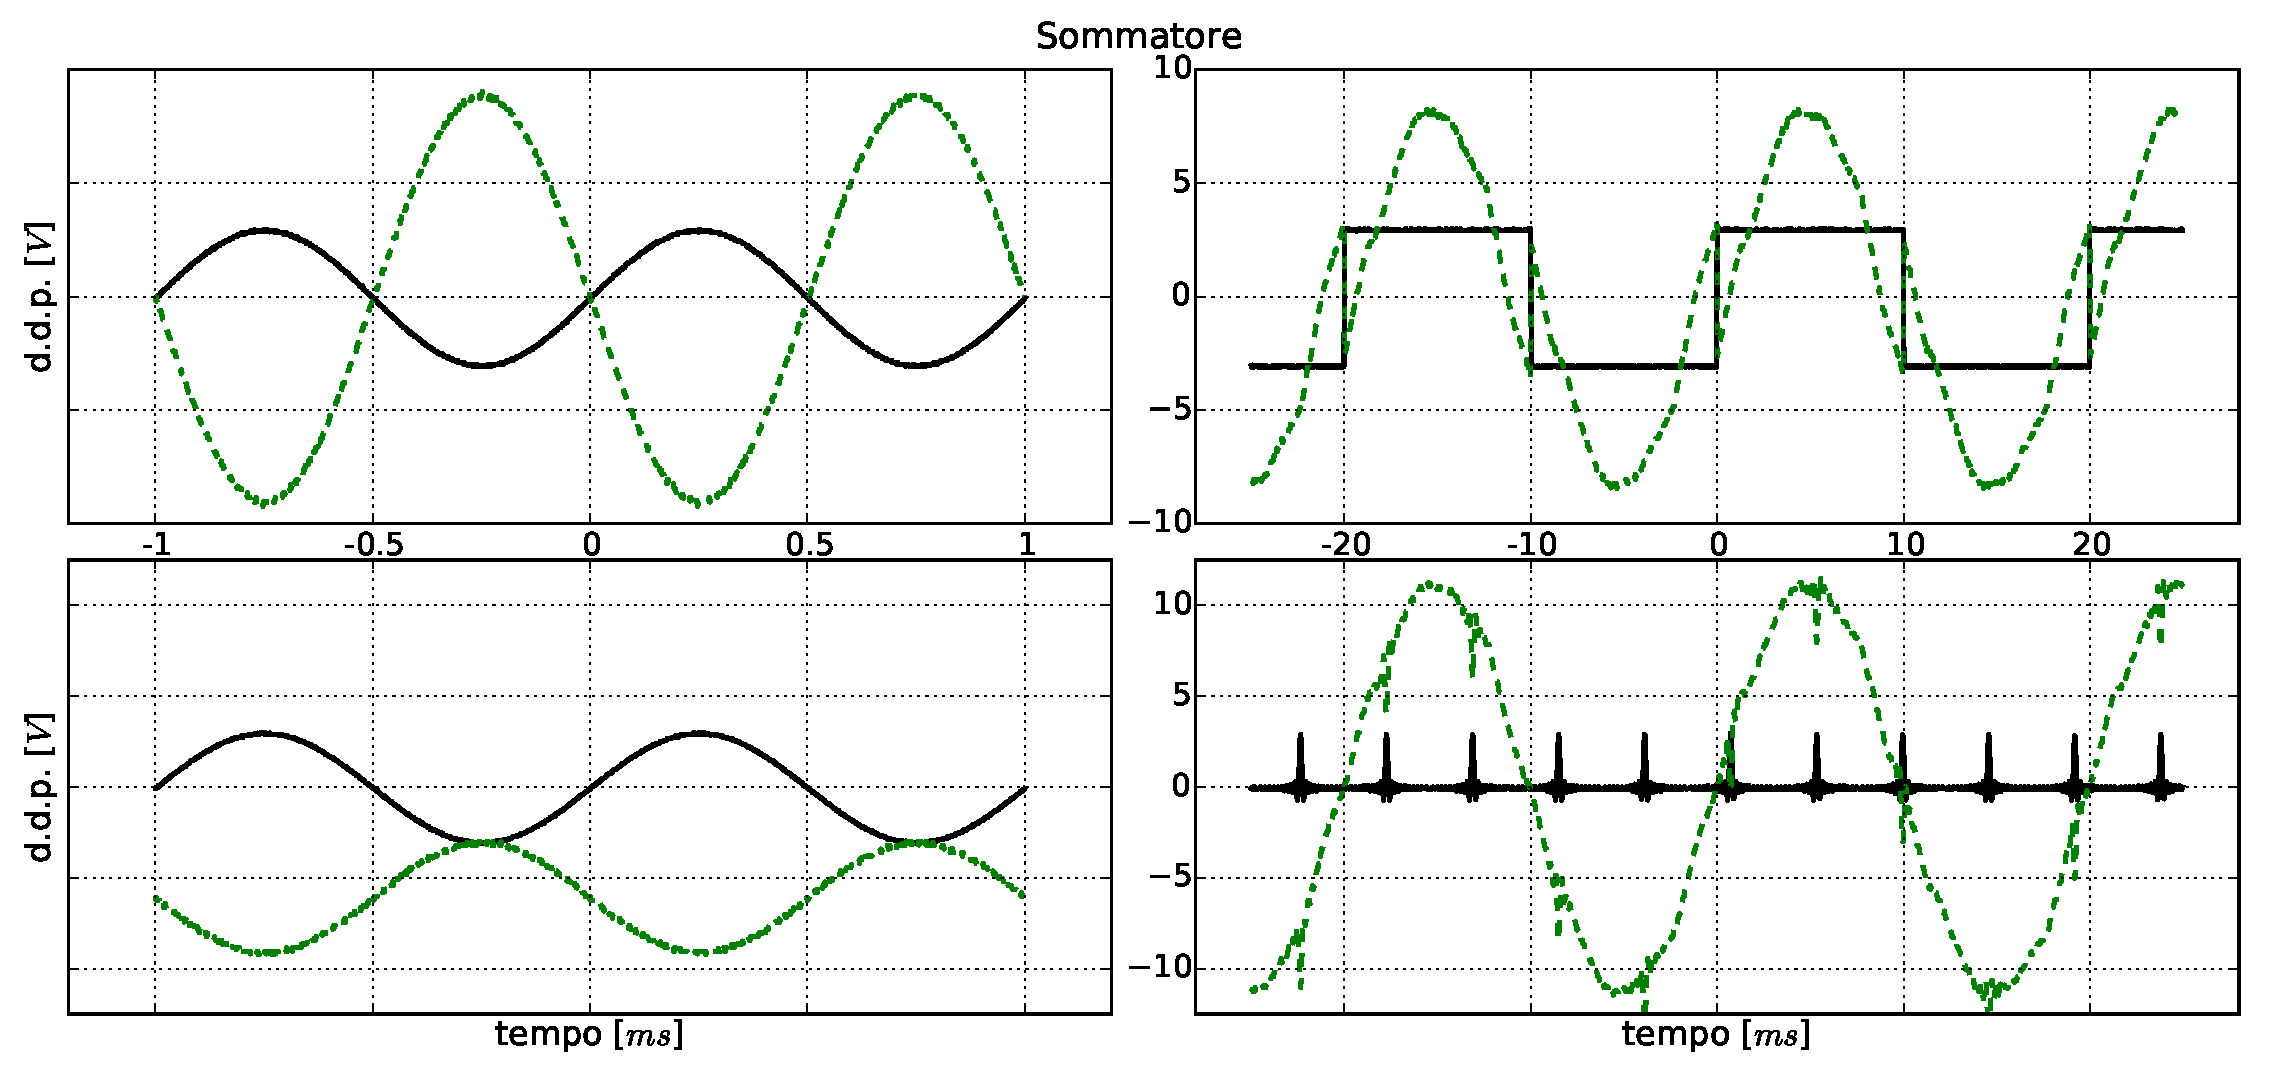
\includegraphics[width=.9\textwidth]{sum_serie_05.pdf}
			\caption{In nero possiamo vedere uno dei segnali in input mentre in verde tratteggiato il segnale in output. Nel primo grafico in alto a sinistra vediamo la somma di tre segnali sinusoidali identici. In quello a destra è stato aggiunto un segnale DC di +6V che evidentemente, per la natura del sommatore, porterà ad un offset di -6V. Nel terzo grafico in basso a sinistra possiamo vedere un'onda sinusoidale con sommata un'onda quadra mentre nell'ultimo grafico abbiamo sommato un cardiode ad una sinusoidale.}
			\label{fig:sum}
\end{figure}

È evidente come il circuito si comporti da sommatore invertente. I valori di resistenza utilizzate sono stati $R_0=(10.01\pm0.02)$ \si{\kilo\ohm}, $R_1=(9.95\pm0.01)$ \si{\kilo\ohm}, $R_2=(10.02\pm 0.01)$ \si{\kilo\ohm} e $R_3=(9.97\pm0.01)$ \si{\kilo\ohm}. \phantom{xxxxxxxxxxxxxxxxxxxxxxxxxxxxxxxxxxxxxxxx}
\begin{wrapfigure}[12]{r}[0pt]{55mm}
	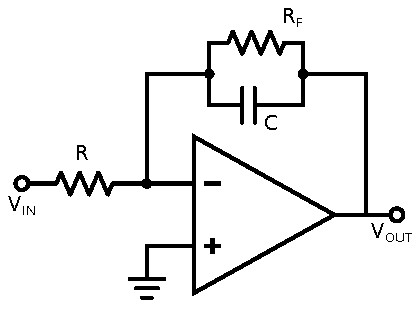
\includegraphics[width=55mm]{ccint.pdf}
	\caption{Circuito integratore}
	\label{fig:ccint}
\end{wrapfigure}

\section{Integratore}

In questa parte dell'esperienza utilizzeremo un op-amp per costruire un circuito integratore. Analizzando lo schema riportato in Fig. \ref{fig:ccint}, assumendo che $R_f=\infty$\footnote{Senza tale approssimazione risulta particolarmente complicata la trattazione del circuito.}, è semplice ricavare $I=C\frac{d(V_A-V_{out})}{dt}$ da cui $V_{in}=-RC\frac{V_{out}}{dt}$.

Vale la seguente relazione:%Non siamo matematici ma la seguente relazione è triviale:

\begin{equation}
V_{out}=-\frac{1}{RC} \int V_{in}dt +costante
\label{eq:int}
\end{equation}

I valori di resistenze e capacità utilizzate sono $R=(99.2 \pm 0.1)$ \si{\kilo\ohm},\\
$R_f=(2.247 \pm 0.001)$ \si{\mega\ohm} e $C=(0.097 \pm 0.002)$ \si{\micro\farad}. 

Poiché nel circuito è presente un condensatore, dobbiamo preoccuparci di calcolare la frequenza di taglio.
Considerando la presenza di un'op-amp e la struttura del circuito, esso funzionerà meglio a frequenze basse che a frequenze alte (un condensatore a basse frequenze si comporta come un circuito aperto, ad alte frequenze come un filo ideale).
Assumendo trascurabili i contributi dati da $R_f$ e dalla resistenza interna dell'oscilloscopio (la prima molto grande, dell'ordine del $\si{\mega\ohm}$, la seconda messa in parallelo con l'impendenza in uscita del'op-amp\footnote{Ricordiamo che l'impedenza in uscita dell'op-amp è praticamente nulla in quanto abbiamo un transistor fet che porta direttamente a ground.}), la frequenza di taglio è stimabile da $f\simeq \frac{1}{2\pi C R_1}$.
Inserendo i valori numerici otteniamo $f \simeq \SI{15}{\hertz}$.
Il circuito si comporterà all'incirca come un filtro passa basso.
Abbiamo dunque deciso di utilizzare dei segnali in ingresso a frequenza di \SI{10}{\hertz}.
Abbiamo tuttavia provato anche per frequenze di \SI{1}{\kilo\hertz}.
I risultati sono esposti nei seguenti grafici.

$$Grafici$$

Come vediamo, anche per alte frequenze rispetto a quella di taglio (100 volte) il circuito funziona ancora come integratore. 
%sebbene ci sia un fattore moltiplicativo inferiore a 1 che modula l'integrale.
Inoltre si noti la presenza di un offset sovrapposto al segnale in uscita. Tale tensione continua è la costante di Eq. \eqref{eq:int}



Abbiamo successivamente provato a togliere la resistenza di feedback $R_f$.
Dalla teoria sappiamo che tale circuito in linea ideale è instabile per frequenze troppo basse, in quanto non abbiamo un circuito di retroazione e dunque non riusciamo a controllare il segnale in output.
In pratica, poichè l'op-amp non è ideale, il circuito non funziona mai.
Infatti, per frequenze alte abbiamo visto in uscita un segnale che cresceva nel tempo.
Pensiamo che il motivo che spiega tale fenomeno sia la non perfetta simmetria dell'amplificatore operazionale.
Se così fosse infatti, avremmo che il condensatore tende a caricari positivamente in quanto il valore di tensione di clapping positivo era, in modulo, maggiore di quello negativo.

\section{Derivatore}

\begin{wrapfigure}[11]{r}[0pt]{65mm}
	\caption{Circuito derivatore}
	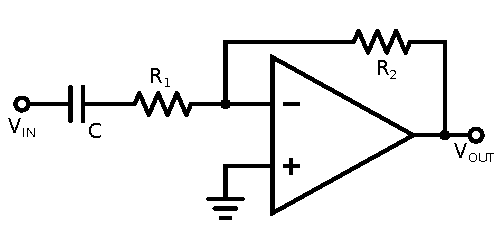
\includegraphics[width=65mm]{ccder.pdf}
	\label{fig:ccder}
\end{wrapfigure}

In quest'ultima parte dell'esperienza analizzeremo il circuito derivatore, il cui schema è riportato in Fig. \ref{fig:ccder}.
Anche in questo caso è banale ricavare l'equazione che lega $V_{out}$ a $V_{in}$: $C\frac{dV_{in}}{dt}=-\frac{V_{out}}{R_2}\Rightarrow V_{out}=-R_2C\frac{dV_{in}}{dt}$.

I valori di resistenze e capacità utilizzati sono $R_2=(9.95 \pm 0.01)$ \si{\kilo\ohm}, $R_1=(1007.9 \pm 0.2)$ \si{\ohm} e $C=(0.097 \pm 0.002)$ \si{\micro\farad}.

Come già fatto per il circuito integratore dobbiamo calcolare la frequenza di taglio prima di poter decidere la frequenza alla quale effettuare le misure.
Risulta immediato dalle considerazioni fatte nella precedente sezione ricavare $f=\frac{1}{2 \pi R^* C}$ con $R^*=R_2+R_1$.
Il valore numerico risulta essere $f \simeq \SI{144}{\hertz}$.
In questo caso è evidente che il segnale sarà smorzato per frequenze inferiori a quella di taglio. Abbiamo effettuato il campionamento alla frequenza di $\SI{100}{\hertz}$, abbastanza vicino alla frequenza di taglio da non avere smorzamenti evidenti.

I risultati sono riportati nel seguente grafico.

\begin{figure}[h]
	\centering
			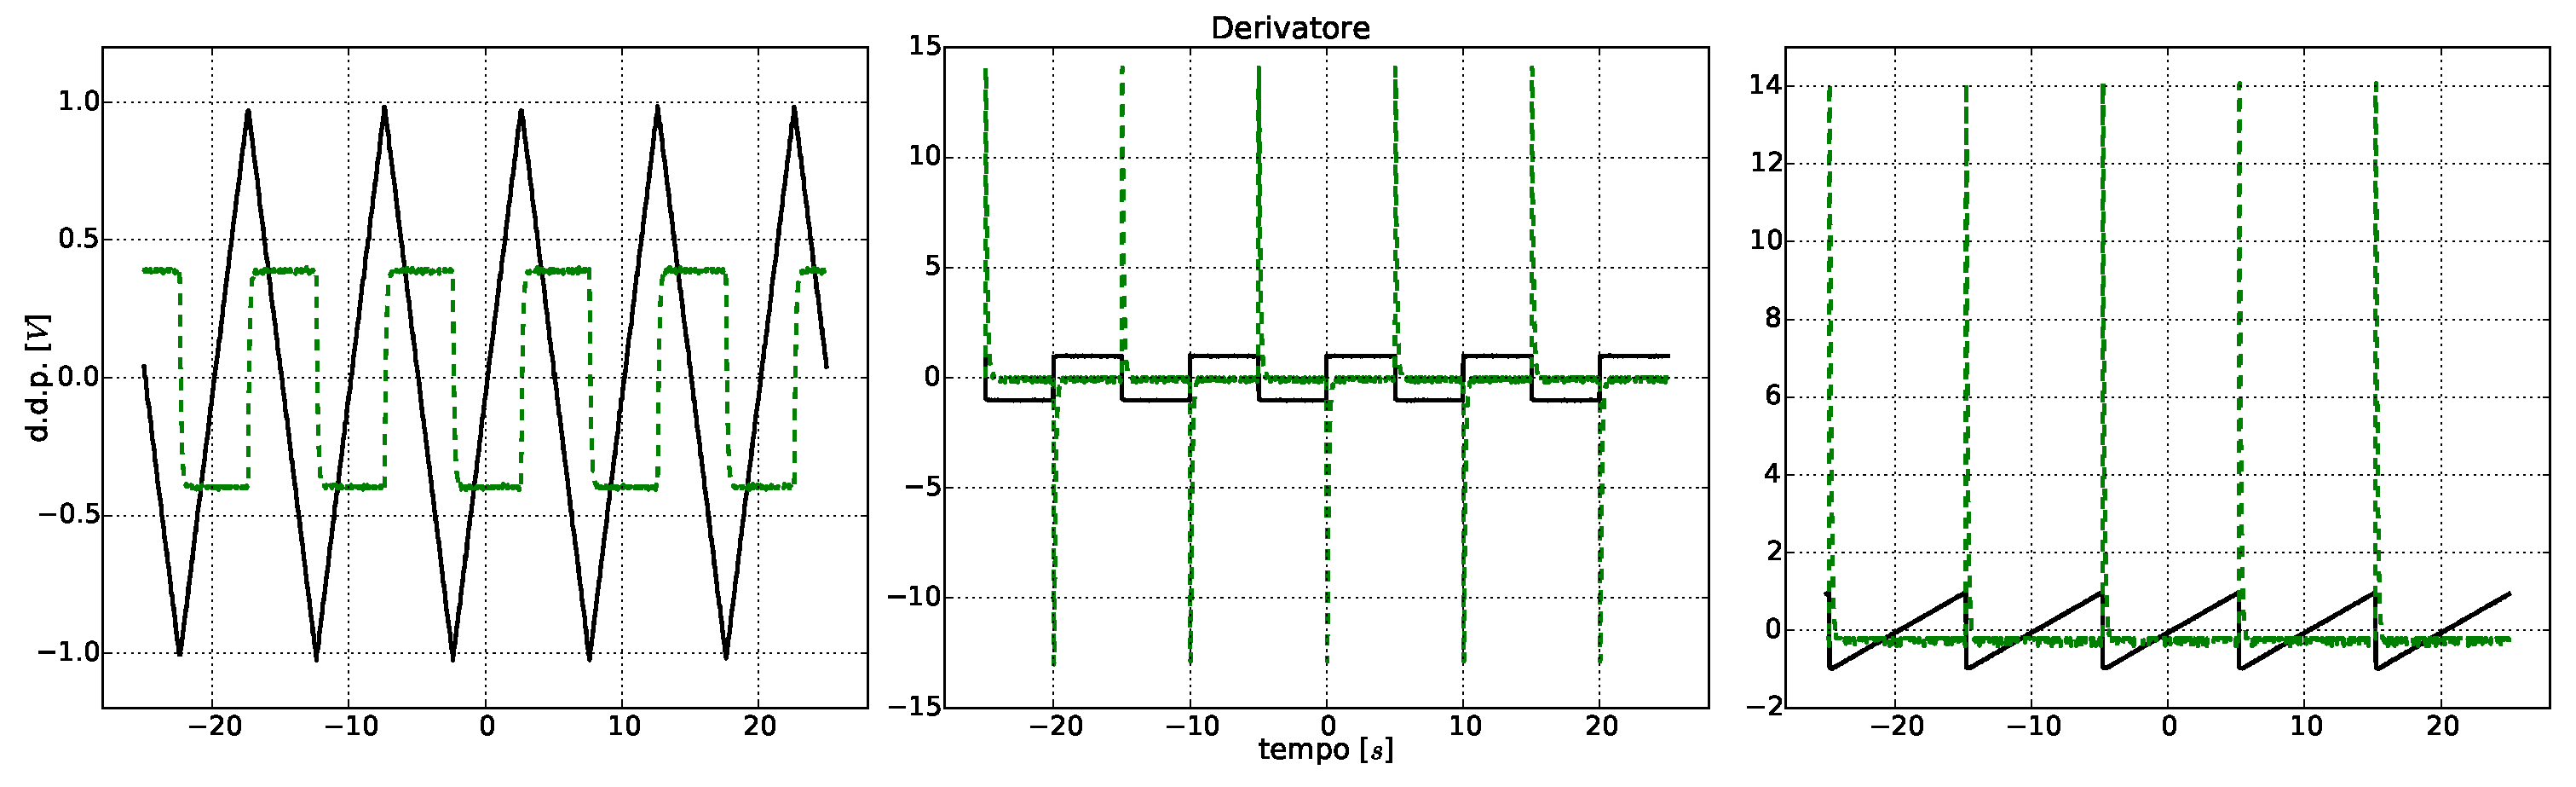
\includegraphics[width=.9\textwidth]{der_serie_10.pdf}
			\caption{Come vediamo graficamente in questo caso non è presente alcun offset in quanto il condensatore taglia i segnali continui in entrata. Inoltre, nel primo grafico in alto a sinistra notiamo come il segnale in output sia amplificato molto di più che negli altri 3 grafici. Ciò è dovuto alla frequenza più alta alla quale è stato eseguito il campionamento.}
			\label{fig:der}
\end{figure}

Abbiamo provato ad aumentare la frequenza e abbiamo notato che il guadagno si stabilizzava su un valore di circa -10.
Questo risultato è coerente con la teoria, in quanto ad alte frequenze l'impedenza del condensatore diventa trascurabile e dunque il circuito diventa simile all'amplificatore invertente studiato nella prima sezione, con la differenza che esso amplifica la derivata del segnale.
\newpage
\noindent \begin{minipage}{\linewidth}
Inoltre notiamo che la fase non è quella tipica del filtro notch già studiato nella precedente esperienza. Questo è dovuto al fatto che noi abbiamo considerato la differenza di fase tra i due segnali ai capi del ponte di Wien, non tra segnale in input e differenza dei due segnali in output. Tale relazione risulta infatti essere:

\begin{equation}
\vartheta_{out|in}=arctan\left[\frac{2 C R \omega \left(C^2 R^2 \omega^2-1\right)}{C^4 R^4 \omega^4+C^2 R^2 \omega^2+1}\right]
\label{teo}
\end{equation}

Poichè non è stata rilevata la differenza di fase direttamente durante l'esperienza, essa è stata calcolata dai dati sperimentali imponendo la condizione, valida per ogni $t$:

\begin{equation}
V_{out}sin(\omega t + \vartheta)=V(CH1)sin(\omega t + \varphi)-V(CH2)sin(\omega t)
\end{equation}

Scegliendo come tempo $t=0$, e applicando un arcoseno, otteniamo subito lo sfasamento del segnale in uscita rispetto a quello in entrata.

\begin{equation}
\vartheta=asin\left(\frac{V(CH1)}{V_{out}}sin(\varphi)\right)
\label{dati}
\end{equation}


Riportiamo in Fig \ref{fig:pahser} la legge teorica (\ref{teo}) e dati sperimentali rielaborati attraverso (\ref{dati}). Nonostante la propagazione degli errori, nel grafico non sono ancora distinguibili le barre d'errore.
\end{minipage}

% questa dovrebbe essere la fase GIUSTA (da mettere a parte) y=180/pi*np.arctan((2*C*R*w*(-1 + (C*R*w)**2))/(1 + (C*R*w)**2 + (C*R*w)**4))

\section{Conclusioni}
\noindent \begin{minipage}{\linewidth}
Attraverso il ponte di Wien siamo riusciti ad ottenere una misura precisa del valore di un capacitore incognito. Un valore compatibile con quello misurato dal multimetro e dichiarato dal costruttore è ottenibile sia dalle equazioni di bilanciamento che dalla loro combinazione. Notiamo dai dati riportati in tabella che quest'ultimo procedimento è quello che permette una stima affetta da minor errore. 
Abbiamo verificato il funzionamento del ponte di Wien come filtro notch. Esso, come già detto, non risulta efficace come un filtro notch costruito utilizzando capacitore in serie ad un'induttanza. Inoltre, per le scelte da noi fatte di resistenze e capacità, l'intensità picco-picco del segnale in output non potrà mai essere superiore a $\frac{V_{in}}{2}$.
\end{minipage}

\begin{figure}[H]%[30]
	\centering
	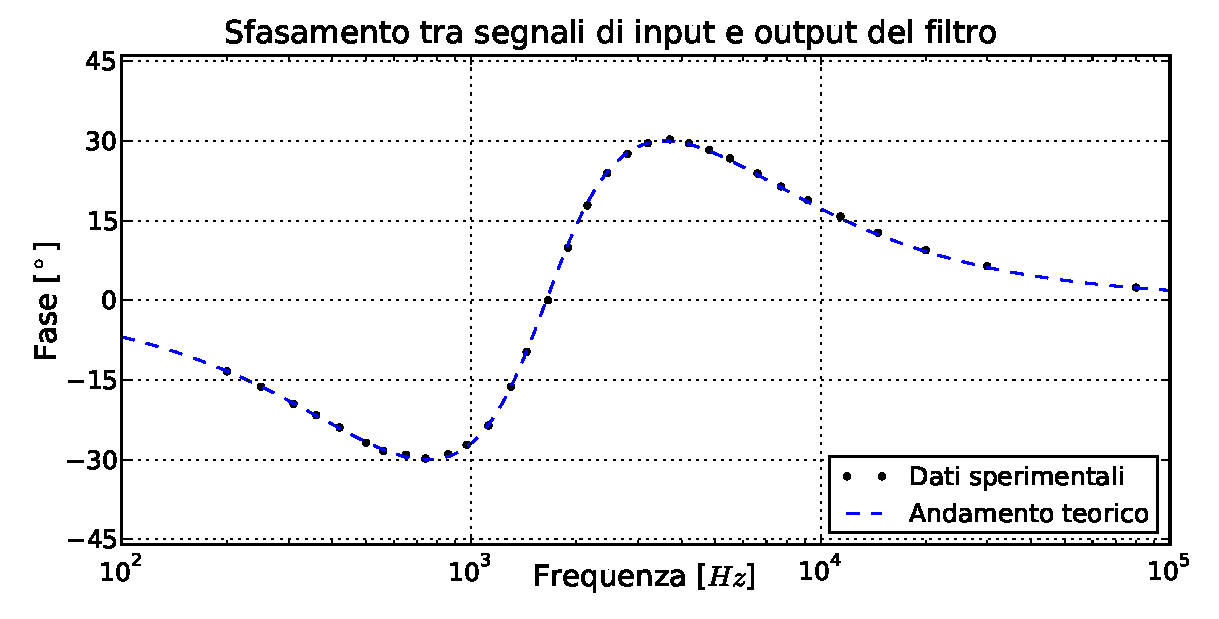
\includegraphics[width=150mm]{i_peli.pdf}
		\caption{Nel grafico sono riportati i valori di differenza di fase tra il segnale in input al circuito e il segnale in output. Ricordiamo che i dati sperimentali sono stati rielaborati usando la formula (\ref{dati}).}
	\label{fig:pahser}
\end{figure}
\end{document}
